\documentclass[a4paper,12pt]{report}
\usepackage[utf8]{inputenc}
\usepackage{imakeidx}
\usepackage{graphicx}
\usepackage{float} %required for the placement specifier H
\usepackage{multicol}		%multicolumns
\usepackage{tabto}

\makeindex[columns=3]

\pagenumbering{roman}

%opening
\title{WolfSSL}
\author{Luca Valentini}
\date{Insert Date}

\begin{document}
\maketitle
\tableofcontents



\newpage
\begin{abstract}
 Explanation of this article. Must be a synthesis
\end{abstract}


\pagenumbering{arabic}
\chapter{SSL Protocol}

\section{Introduction}
The SSL protool is a client/server protocol that provides the following basic security services to the communicating peers:
\begin{itemize}
	\item Authentication (both peer entity anda data origin authentication) services
	\item Connection confidentiality services
	\item Connection integrity services
\end{itemize}

The SSL protocol is sockets-oriented, meaning that all or none of the data that is sent to or received from a network connection is cryptographically protected in exactly the same way. It can be best viewed as an intermediate layer between the transporrt and the application layer that serves two purposes:
\begin{itemize}
	\item Establish a secure connection between the commucating peers
	\item Use this connection to securely trasmit giher-layer protocol data from the sender to the reciever. It therefore fragments the data in pieces called fragments; each fragment is optionally compressed, authenticated, encrypted, prepended with a header, and transmitted to the reciever. Each data fragment prepared this way is sent in a distinct SSL record.
\end{itemize}

\begin{figure}[H]
    \centering
    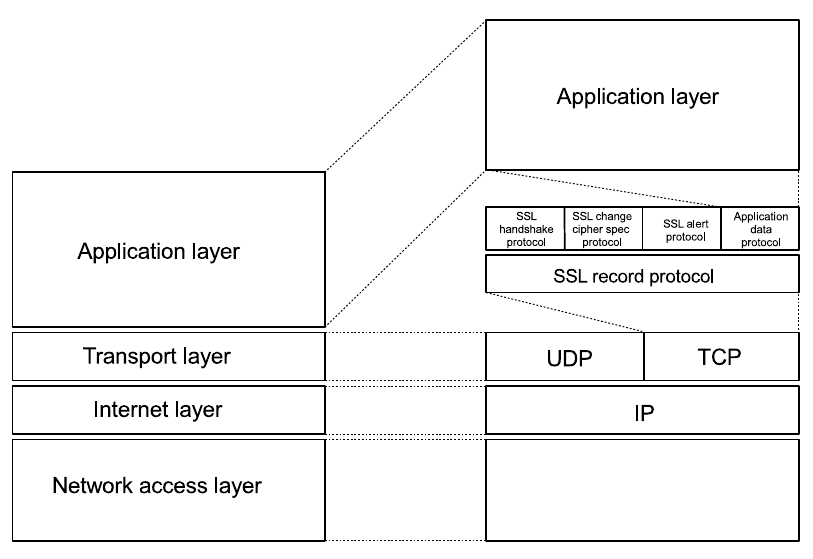
\includegraphics[scale=0.5]{subLayer_subProtocols.png}
    \caption{The SSL with its (sub)layer and (sub)protocols}
    \label{fig:galaxy}
\end{figure}

The SSL consists of two sublayers and a few subprotocols:
\begin{itemize}
	\item The lower sublayer is stacked on top of some connection-oriented and reliable transport layer protocol. This layer basically comprises the SSL record protocol that is used for the encapsulation of the higher-layer protocol data.
	\item The higher sublayer is stacked on top of the SSL record protocol and comprises four subprotocols.

	\begin{itemize}
		\item The \emph{SSL handshake protocol} is the core subprotocol of SSL. It is used for establishment of a secure connection. It allows the communicating peers to authenticate each other and to negotiate a cipher suite and a compression method.
		\item The \emph{SSL change cipher spec protocol} is used to put the parameters, set by the SSL handshake protocol in place and make them effective.
		\item The \emph{SSL alert protocol} allows the communicating peers to signal indicators of potential problems and send respective alert messages to each other.
		\item The \emph{SSL application data protocol} is used for the secure transmission of application data.
	\end{itemize}

\end{itemize}

In spite of the fact that SSL consists of several subprotocols, we use the term \emph{SSL protocol} to refer to all of them simultaneously.

\section{SSL Handshake}
The SSL handshake protocol is layered on top of the SSL record protocol. It allows a client and server to authenticate each other and to negotiate issues like cipher suites and compression methods.

\begin{figure}[H]
    \centering
    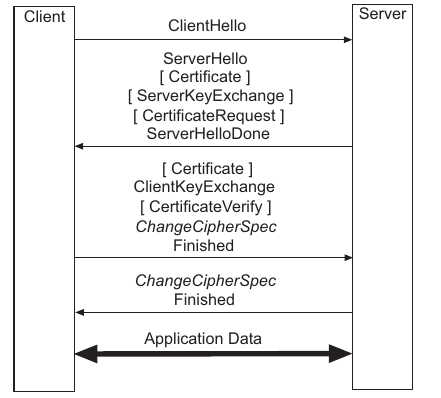
\includegraphics[scale=0.7]{handshake.png}
    \caption{The SSL handshake protocol}
    \label{fig:galaxy}
\end{figure}

\vspace{5mm} %5mm vertical space
The SSL handshake protocol comprises four sets of messages:
\begin{itemize}
\item The first flight comprises a single \emph{ClientHello} message that is sent from the client to the server.
\item The second flight comprises two messages that are sent back from the server to the client:
\begin{enumerate}
\item \emph{ServerHello} message is sent in response to the \emph{ClientHello} message
\item (optional) If the server is to authenticate itself, it may send a \emph{Certificate} message to the client.
\item (optional) Under some circumstances, the server may send a \emph{ServerKeyExchange} message to the client.
\item (optional) If the server requires the client to authenticate itself with a public key certificate, then it may send a \emph{CertificateRequest} message to the client.
\item Finally, server send a \emph{ServerHelloDone} message to the client.
\end{enumerate}
\item The third flight comprises three to five messages that are again sent from the client to the server:
\begin{enumerate}
\item (optional) If the server has sent a \emph{CertificateRequest} message, then the client sends a \emph{Certificate} message to the server.
\item In the main step of the protocol, the client sends a \emph{ClientKeyExchange} message to the server.
\item (optional) If the client has sent a certificate to the server, then it must also send a \emph{CertificateVerify} message to the server. This message is digitally signed with the private key that corresponds to the client certificate's public key.
\item The client sends a \emph{ChangeCipherSpec} message to the server (using the SSL change cipher spec protocol) and copies its pending write state into the current write state.
\item The client sends a \emph{Finished} message to the server. As mentioned above, this is the first message that is cryptographically protected under the new cipher spec.
\end{enumerate}
\item The fourth flight comprises two messages that are sent from the server back to the client:
\begin{enumerate}
\item The server sends another \emph{ChangeCipherSpec} message to the client and copies its pending write state into the current write state.
\item Finally, the server send a \emph{Finished} message to the client. Again, this message is cryptographically protected under the new cipher spec.

\end{enumerate}
\end{itemize}

At this point in time, the SSL handshake is complete and the client and server may start exchanging application-layer data.

\chapter{Wolf SSL}
The wolfSSL embedded SSL library is a lightweight SSL/TLS library written in ANSI C and targeted for embedded, RTOS, and resource-constrained
environments - primarily because of its small size, speed, and feature set.
\\It's free and it has an excellent cross platform support.
\\WolfSSL supports standards up to the current TLS 1.3 and DTLS 1.2 levels, is up to
20 times smaller than OpenSSL and it's powered by the colfCrypt library.

\vspace{5mm} %5mm vertical space
This library is built for maximum portability and supports the C programming language as a primary interface. It also supports several other host languages, including Java (wolfSSL JNI), C\# (wolfSSL C\#), Python, and PHP and Perl.

\vspace{5mm} %5mm vertical space
To improve performance it supports hardware cryptography and acceleration on several platforms.

\vspace{5mm} %5mm vertical space
In the following list you can see some of WolfSSI’s features:
\begin{itemize}
\item Runtime memory usage between 1-36 kB
\item OpenSSl compatibility layer
\item Hash Functions: \begin{multicols}{3}\begin{itemize}
\item MD2
\item MD4
\item MD5
\item SHA-1
\item SHA-224
\item SHA-256
\item SHA-384
\item SHA-512
\item BLAKE2b
\item RIPEMD-160
\item Poly1305
\end{itemize}
\end{multicols}
\item Mutual authentication support (client/server)
\item SSL Sniffer (SSL Inspection) Support
\item IPv4 and IPv6 support


\end{itemize}

\cleardoublepage
The operating systems supported are:
\begin{multicols}{3}
\begin{enumerate}
\item Win32/64 \item Linux \item Mac OS X \item Solaris \item ThreadX \item VxWorks \item FreeBSD \item NetBSD \item OpenBSD \item embedded Linux \item Yocto Linux \item OpenEmbedded \item WinCE \item Haiku \item OpenWRT \item iPhone(iOS) \item Android \item Nintendo Wii and Gamecube through DevKitPro \item QNX \item MontaVista \item NonStop \item TRON / ITRON /  ITRON \item Micrium  C / OS - III \item FreeRTOS \item SafeRTOS \item NXP / Freescale MQX \item Nucleus \item TinyOS \item HP / UX \item AIX \item ARC MQX \item TI - RTOS \item uTasker \item embOS \item INtime \item Mbed \item uT - Kernel \item RIOT \item CMSIS -RTOS \item FROSTED \item Green Hills INTEGRITY \item Keil RTX \item TOPPERS \item PetaLinux \item Apache Mynewt \item PikeOS 
\end{enumerate}
\end{multicols}

\chapter{Test case}
\section{Client/Server provided by WolSSL}

\begin{figure}[H]
    \centering
    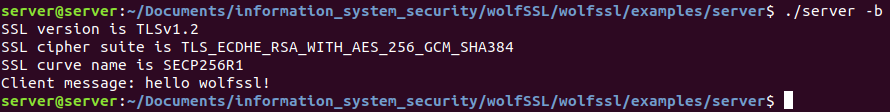
\includegraphics[scale=0.5]{test/examples/client-server/server.png}
    \caption{Server SSL}
    \label{fig:galaxy}
\end{figure}

\begin{figure}[H]+
    \centering
    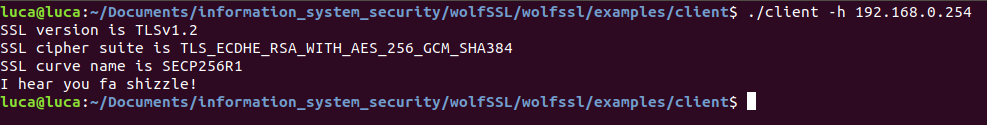
\includegraphics[scale=0.45]{test/examples/client-server/client.png}
    \caption{Client SSL}
    \label{fig:galaxy}
\end{figure}

In this example, the server is a simple SSL server that allows only one client connection; after the connection with a client, the server receives an encrypted message from client, it responds and quits.
\\The -b parameter allows the server to bind to any interface instead of localhost only.
\\
\\The client after the connection with the server, sends a message (hello wolfssl!) and after the server response, it quits.
\\The -h parameter allows the client to specify the server address to perform the connection.

\begin{figure}[H]
    \centering
    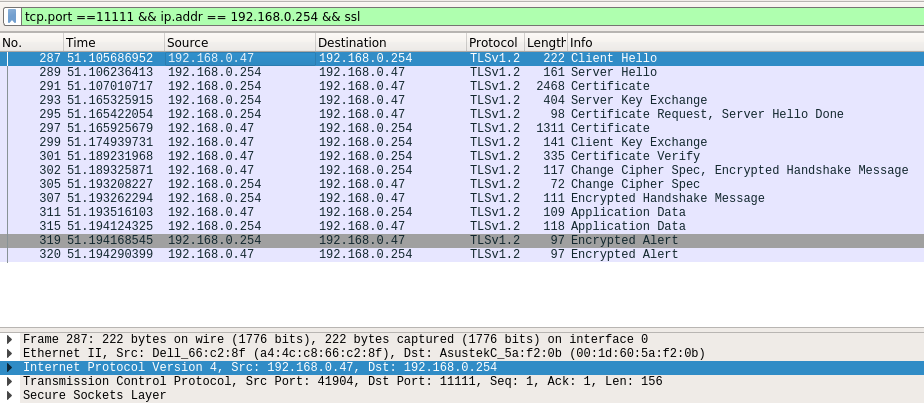
\includegraphics[scale=0.5]{test/examples/client-server/wireshark1.png}
    \caption{All SSL packets sent}
    \label{fig:galaxy}
\end{figure}
Client IP:  192.168.0.47 \hspace{4cm} Server IP: 192.168.0.254\\ \\
Come si puo' bene vedere dalla figura soprastante, la comunicazione viene iniziata dal client con un 'Client Hello'; dopo SSL handshake, ci sono due messaggi 'Application Data' inviati rispettivamente dal client verso il server e dal server verso il client il cui contenuto e' cifrato. Una volta che il server invia la risposta al client, la comunicazione viene chiusa attraverso 'Encrypted Alert'.

\begin{figure}[H]
    \centering
    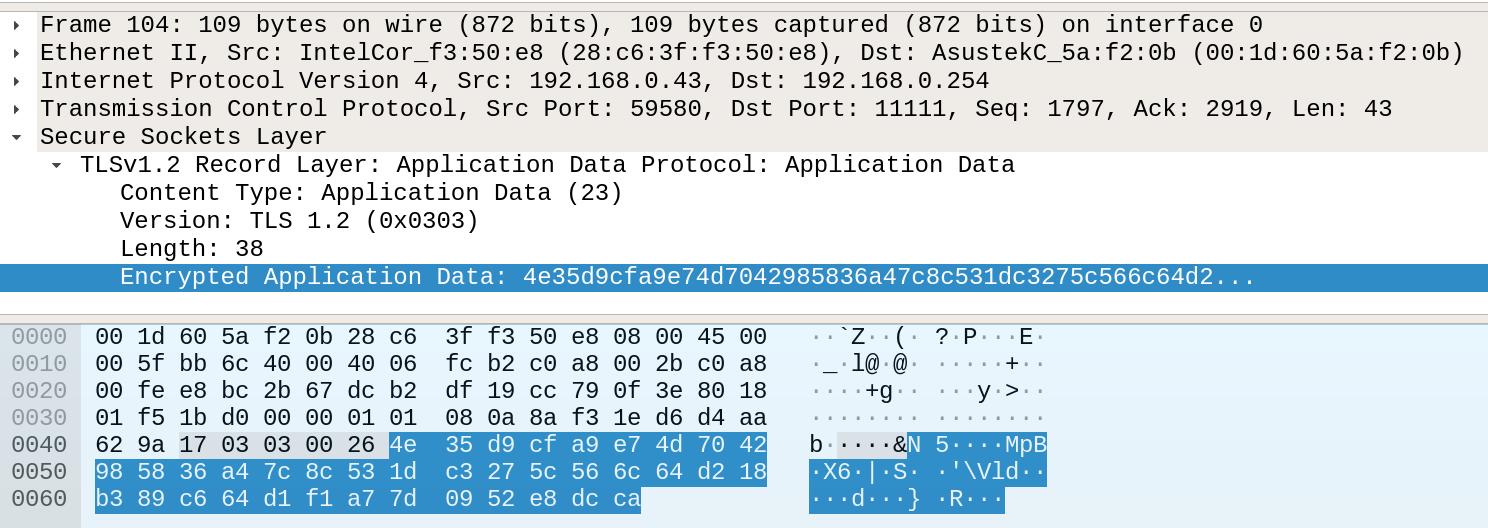
\includegraphics[scale=0.3]{test/examples/client-server/encrypted_data.png}
    \caption{Content of the encrypted message}
    \label{fig:galaxy}
\end{figure}

Come si puo' vedere, lo scambio di messaggi e' cifrato.


\pagebreak

\section{EchoClient/EchoServer provided by WolfSSL}
\begin{figure}[H]
\hspace*{-1cm}     
    \centering
    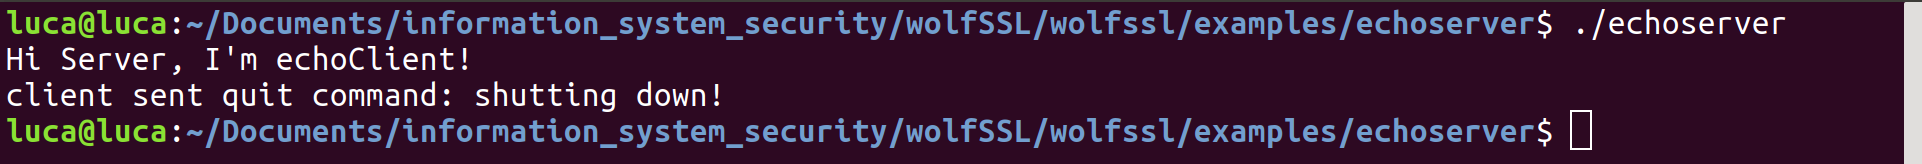
\includegraphics[scale=0.25]{test/examples/echoclient-echoserver/echoServer.png}
    \caption{EchoServer SSL}
    \label{fig:galaxy}
\end{figure}

\begin{figure}[H]
\hspace*{-1cm}     
    \centering
    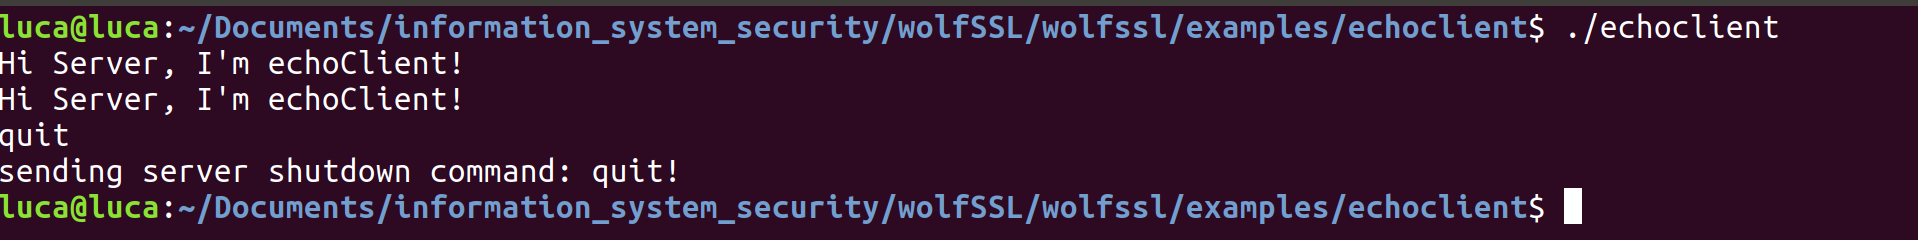
\includegraphics[scale=0.25]{test/examples/echoclient-echoserver/echoClient.png}
    \caption{EchoClient SSL}
    \label{fig:galaxy}
\end{figure}

\begin{figure}[H]
\hspace*{-2cm}     
    \centering
    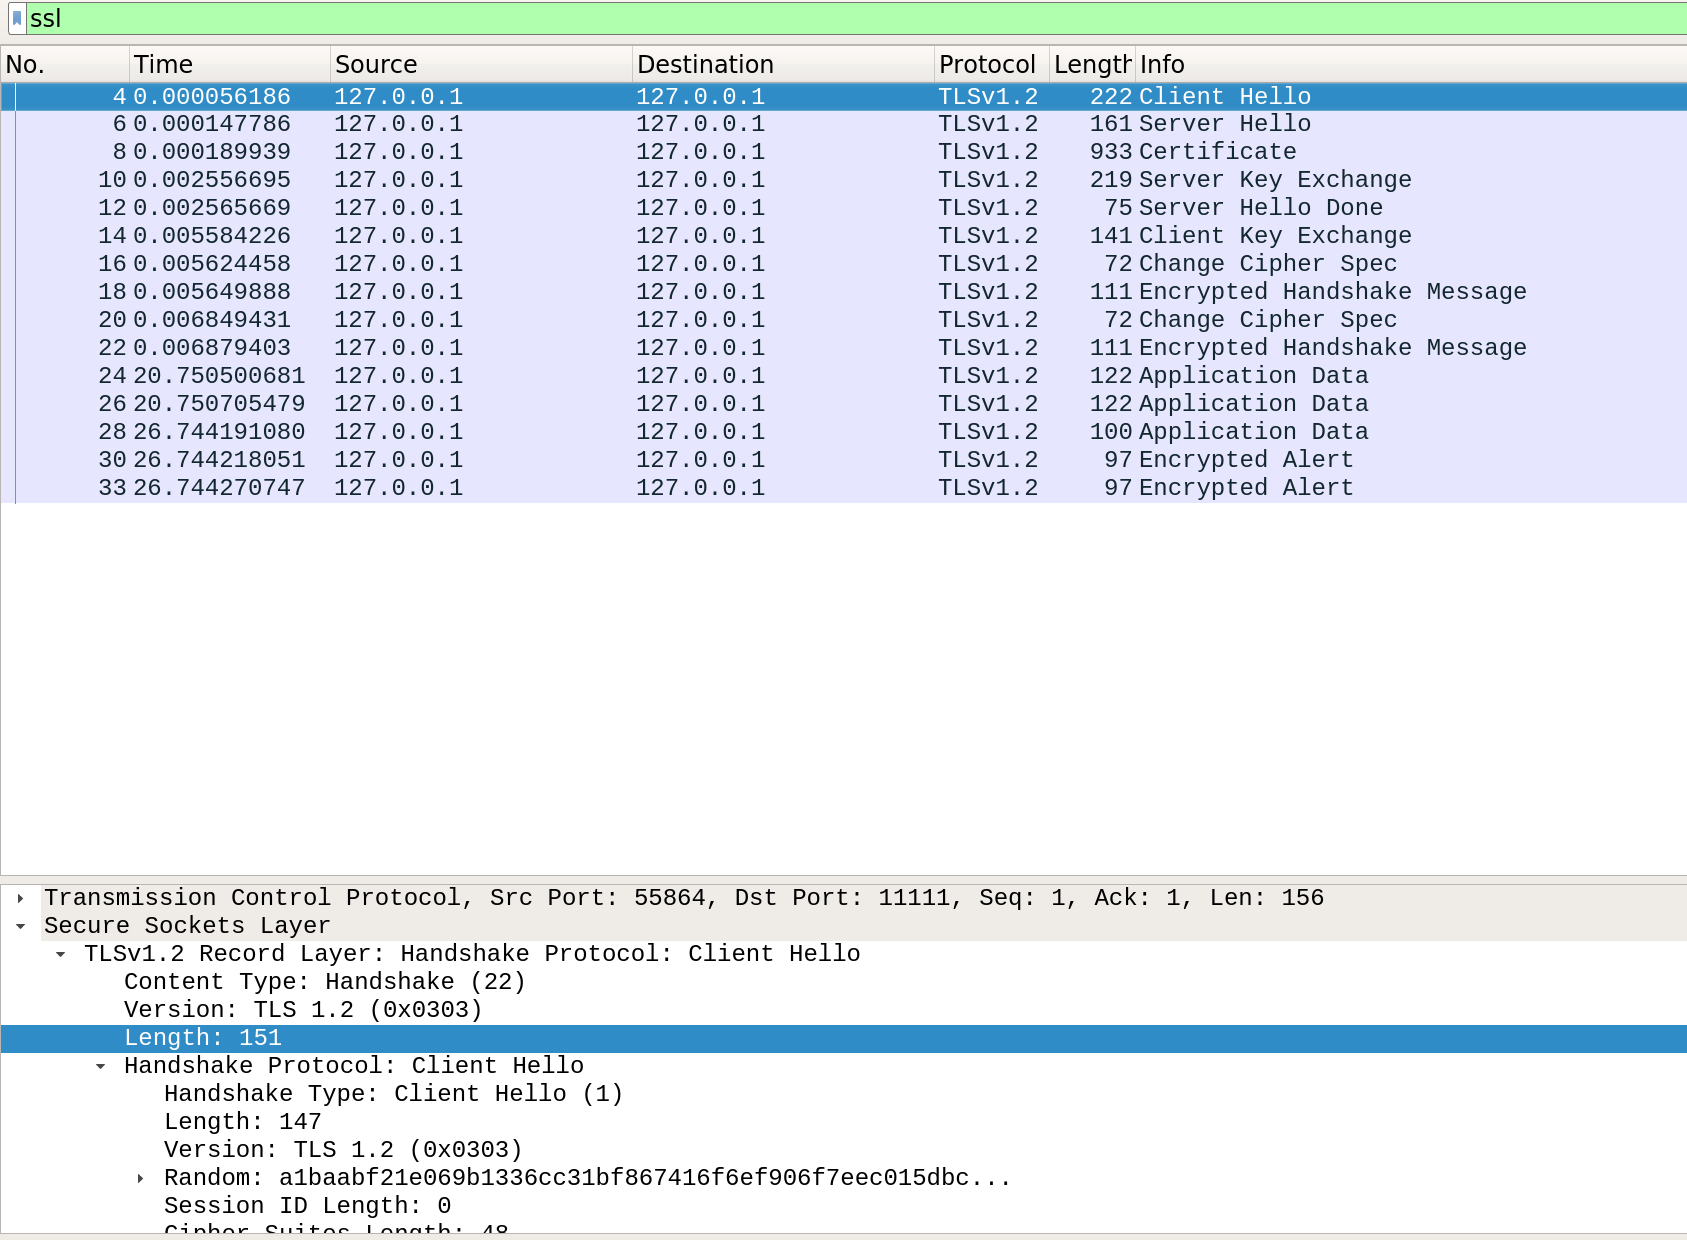
\includegraphics[scale=0.3]{test/examples/echoclient-echoserver/wireshark.png}
    \caption{All SSL packets sent}
    \label{fig:galaxy}
\end{figure}


\end{document}
